\usetikzlibrary{arrows}
\usetikzlibrary{decorations.pathreplacing}

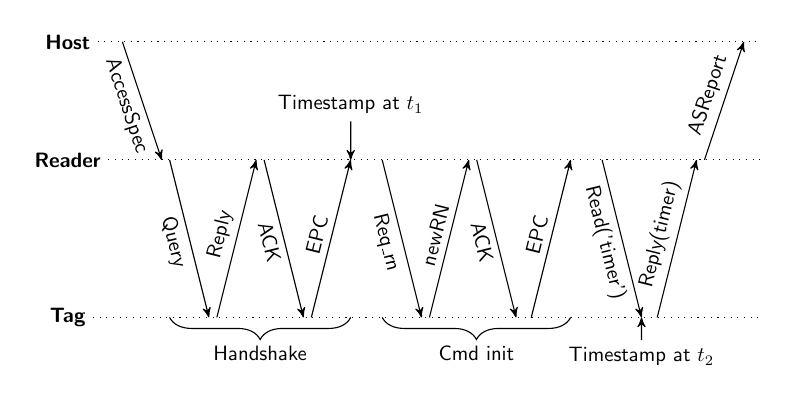
\begin{tikzpicture}[font=\sffamily,
>=stealth',
commentl/.style={text width=3cm},
scale=1.0, 
every node/.style={scale=0.75}]
\tikzstyle{myedgestyle} = [dotted]
\tikzstyle{ar} = [->]
\node(host) at (-0.5,3.5cm){\textbf{Host}};
\draw [myedgestyle] (host) edge ([xshift=8.8cm]host);
\node(reader) at (-0.5,2cm){\textbf{Reader}};
\draw [myedgestyle] (reader) edge ([xshift=8.8cm]reader);
\node(tag) at (-0.5,0cm){\textbf{Tag}};
\draw [myedgestyle] (tag) edge ([xshift=8.8cm]tag);
\node(h) at (-0.4,3.5cm){};
\node(r) at (-0.4,2cm){};
\node(t) at (-0.4,0cm){};

\draw[ar] ([xshift=5mm]h.east) coordinate(as1) --
([xshift=10mm]r.east) coordinate(as2) node[midway, below, sloped]     { AccessSpec};
\draw[ar] ([xshift=1mm]as2.east) coordinate(Q1)--
([xshift=16mm]t.east) coordinate(Q2) node[midway, below, sloped]     { Query};
\draw[ar] ([xshift=1mm]Q2.east) coordinate(R1)--
([xshift=11mm]Q1.east) coordinate(R2) node[midway, above, sloped]     { Reply};
\draw[ar] ([xshift=1mm]R2.east) coordinate(A1)--
([xshift=11mm]R1.east) coordinate(A2)node[midway, below, sloped]     { ACK};
\draw[ar] ([xshift=1mm]A2.east) coordinate(E1)--
([xshift=11mm]A1.east)coordinate(E2) node[midway, above, sloped]     { EPC};
\draw[ar] ([xshift=4mm]E2.east)coordinate(Rq1)--
([xshift=14mm]E1.east)coordinate(Rq2) node[midway, below, sloped]     { Req\_rn};
\draw[ar] ([xshift=1mm]Rq2.east)coordinate(nR1)--
([xshift=11mm]Rq1.east)coordinate(nR2) node[midway, above, sloped]     { newRN};
\draw[ar] ([xshift=1mm]nR2.east)node (A1) {}--
([xshift=11mm]nR1.east)node (A2) {} node[midway, below, sloped]     { ACK};
\draw[ar] ([xshift=1mm]A2.east)coordinate(Er1)--
([xshift=11mm]A1.east)coordinate(Er2) node[midway, above, sloped]     { EPC};
\draw[ar] ([xshift=4mm]Er2.east)coordinate(c1)--
([xshift=14mm]Er1.east)coordinate(c2) node[midway, below, sloped]     { Read('timer')};
\draw[ar] ([xshift=2mm]c2.east)coordinate(r1)--
([xshift=12mm]c1.east)coordinate(r2) node[midway, above, sloped]     { Reply(timer)};
\draw[ar] ([xshift=1mm]r2.east)coordinate(AR1)--
([xshift=6mm,yshift=1.5cm]r2.east)coordinate(AR2) node[midway, above, sloped] { ASReport};


\tikzstyle{br} = [decorate, decoration={brace, amplitude=8pt}]
\draw[br] ([xshift=5mm]E1) -- ([xshift=-5mm]Q2) node[midway, , sloped,yshift=-6mm] {Handshake};
\draw[br] ([xshift=5mm]Er1) -- ([xshift=-5mm]Rq2) node[midway, , sloped,yshift=-6mm] {Cmd init};
%\draw[br] ([xshift=5mm]r1) -- ([xshift=-5mm]c2) node[midway, , sloped,yshift=-6mm] {Cmd};
%\draw[br] ([xshift=5mm,yshift=-6mm]r1) -- ([xshift=-5mm,yshift=-6mm]Rq2) node[midway, , sloped,yshift=-6mm] {Optional};

% Timestamp stuff:
\node(tTag) at ([yshift=-5mm,xshift=0mm]c2.east){Timestamp at $t_2$};
\draw[ar] ([yshift=-15mm,xshift=2mm]tTag)--
([xshift=0mm]c2.east) node[near start]     {};

\node(tReader) at ([xshift=0mm,yshift=7mm]E2.east) {Timestamp at $t_1$};
\draw[ar] (tReader)--
([xshift=0mm]E2.east) node[near start]     {};

\end{tikzpicture}